\documentclass[12pt, a4paper]{article}
\usepackage[margin = 2cm]{geometry}
\pagenumbering{gobble}
\usepackage[T1]{fontenc}   % Pipe symbol
% Vertical text spacing
\parindent = 0cm \parskip = 0cm
% Section
\usepackage[compact]{titlesec} \titlespacing*{\section}{0pt}{2ex}{2ex}
\titleformat*{\section}{\normalfont\Large\bfseries\color[RGB]{0,0,192}}
\titleformat*{\subsection}{\normalfont\bfseries\color[RGB]{192,0,0}}
% Table spacing
\newcommand\TS{\rule{0pt}{2.6ex}}         % Top strut
\newcommand\BS{\rule[-0.9ex]{0pt}{0pt}}   % Bottom strut
\usepackage{array, multirow}
\newcolumntype{L}[1]{>{\raggedright\let\newline\\\TS\BS\arraybackslash}m{#1}}   % Align left
\newcolumntype{C}[1]{>{\centering  \let\newline\\\TS\BS\arraybackslash}m{#1}}
\newcolumntype{R}[1]{>{\raggedleft \let\newline\\\TS\BS\arraybackslash}m{#1}}   % Align right
% Equations
\usepackage{amsmath, bm, bbold, tikz}

\title{CO395 Group 57 \vspace{-1ex}}
\author{Dongxiao Huang, Zheng Xun Phang, Yufeng Zhang}
\date{\vspace{-1.5ex}}

\begin{document}
\maketitle
\section*{Implementation}
\subsection*{Cross-validation}
The entire training data set is divided by 10 to acquire the number of data in each fold of cross validation. Then for each round i of 10 times, the training data set is split into two sections. One called training data set is a set of data with indexes in the i$^{th}$ fold, and another called test data set is a set of data with indexes in the remaining 9 folds. The training data set is used as examples and binary targets to construct the decision tree, while the test data set as only examples in order to get the labels to compute error rate. Finally, an average error estimate is calculated by 10 error rates.
\subsection*{Best-attribute selection}
How do we select the best attribute at each node? For all attributes, we compute the information gain if the dataset is split on that attribute:
\begin{align*}
    \text{Gain(Attribute)} &= \mathcal{I}(p, n) - \left[ \frac{p_0 + n_0}{p + n} \, \mathcal{I}(p_0, n_0) + \frac{p_1 + n_1}{p + n} \, \mathcal{I}(p_1, n_1) \right] \\[0.5ex]
    p_k &= \text{Number of positive examples with attribute} = k \\
    n_k &= \text{Number of negative examples with attribute} = k \\
    p &= p_0 + p_1 = \text{Number of positive examples before split} \\
    n &= n_0 + n_1 = \text{Number of negative examples before split}
\end{align*}
There are two common ways to measure information.
\begin{flalign*}
    &\text{Entropy:} & \mathcal{I}(p, n) &= - \frac{p}{p+n} \log \frac{p}{p+n} - \frac{n}{p+n} \log \frac{n}{p+n} \qquad \text{if } p, n \neq 0 &\\
    & & \mathcal{I}(p, 0) &= \mathcal{I}(0, n) = 0 &\\[0.5ex]
    &\text{Gini impurity:} & \mathcal{I}(p, n) &= \frac{p}{p+n} \left( 1 - \frac{p}{p+n} \right) + \frac{n}{p+n} \left( 1 - \frac{n}{p+n} \right)
\end{flalign*}
We used entropy since it is stated in the specification, but Gini impurity is faster to compute. Both metrics should give similar results since their graphs have a similar shape:
\begin{center}
\begin{minipage} {0.45 \textwidth}
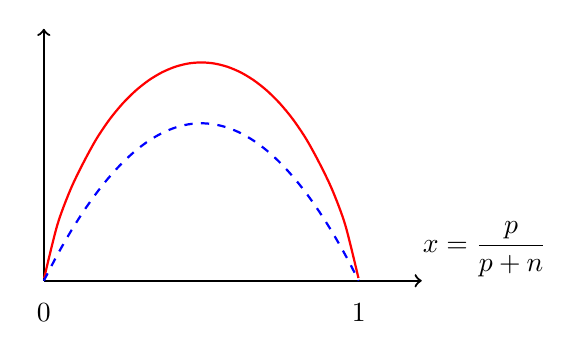
\begin{tikzpicture} [xscale = 4, yscale = 4]
    \draw[->, thick] (0, 0) -- (1.2, 0); 
    \node at (1.4, 0.1) {$\displaystyle x = \frac{p}{p+n}$};
    \draw[->, thick] (0, 0) -- (0, 0.8);
    \newcommand{\gini}[2]    {plot[smooth, domain = #1:#2] (\x, {2 * \x * (1-\x)}) };
    \newcommand{\entropy}[2] {plot[smooth, domain = #1:#2] (\x, {-\x * ln(\x) - (1-\x) * ln(1-\x)}) };
    \draw[thick, red] \entropy{0.001}{0.999};
    \draw[dashed, thick, blue] \gini{0}{1};
    \node at (0, -0.1) {0};
    \node at (1, -0.1) {1};
\end{tikzpicture}
\end{minipage}
\begin{minipage} [b] {0.4 \textwidth}
    {\color{red} Entropy: $-x \log x - (1-x) \log (1-x)$} \\
    \\
    {\color{blue} Gini: $2x (1-x)$}
\end{minipage}
\end{center}
N.B. The \textit{height} of those graphs is irrelevant because minimizing a function is equivalent to minimizing any positive multiple of that function. What matters is their \textit{shape}.\par
\bigskip
The decision tree algorithm is given in the specification, so it's unnecessary to repeat it here. We try to use NumPy functions instead of Python loops for performance since the former run on vectorized C code.\par
\bigskip
To evaluate our decision tree, we performed $K$-fold cross validation as follows:
\begin{enumerate}
    \item Shuffle the dataset and split it into $K = 10$ parts
    \item For each $k \in \{1, \dotsm, K\}$ we train the decision tree on the dataset \textit{excluding} part $k$ and then test the decision tree on part $k$. During testing, we aggregate the predictions from 6 trees (more details later) and increment the relevant cells in the confusion matrix.
\end{enumerate}

\section*{Evaluation}
Each cell of the confusion matrix is a total, not an average, over all folds of cross validation. There were $n = 1000$ test examples in total.\par
\bigskip
\textbf{Note}: It makes no sense to compute classification rate for each emotion separately. For example, if the actual emotion is Anger then (Fear, Surprise) counts as a true negative for Anger even though it's a misclassification.
\bigskip
\subsection*{Clean Data}
\begin{center}
\begin{tabular} { C{2.7cm} | C{1.5cm} C{1.5cm} C{1.3cm} C{1.7cm} C{1.5cm} C{1.5cm} }
\multirow{2}{*}{Actual Class} & \multicolumn{6}{c}{Predicted Class} \\
    & Anger & Disgust & Fear & Happiness & Sadness & Surprise \\ \hline
    Anger     & 106 &  11 &  3 &   5 &  5 &   1 \\
    Disgust   &  23 & 157 &  1 &   5 &  9 &   3 \\
    Fear      &  17 &   2 & 77 &   2 &  7 &  13 \\
    Happiness &  22 &   6 &  1 & 179 &  6 &   1 \\
    Sadness   &  34 &  11 &  3 &   4 & 78 &   2 \\
    Surprise  &  27 &   3 &  7 &   4 &  4 & 161
\end{tabular}
\end{center}
We add up the relevant cells in the confusion matrix above to compute these summary statistics:
\begin{center}
\begin{tabular} { C{2.7cm} | C{1.5cm} C{1.5cm} C{1.3cm} C{1.7cm} C{1.5cm} C{1.5cm} }
    & Anger & Disgust & Fear & Happiness & Sadness & Surprise \\ \hline
    Precision & 0.463 & 0.826 & 0.837 & 0.899 & 0.716 & 0.890 \\
    Recall    & 0.809 & 0.793 & 0.653 & 0.833 & 0.591 & 0.782 \\
    $F_1$ score & 0.589 & 0.809 & 0.733 & 0.865 & 0.647 & 0.832 \\
\end{tabular}
\[ \text{Classification rate} = \frac{106 + 157 + \dotsm + 161}{1000} = 0.758 \]
\end{center}

\subsection*{Noisy Data}
\begin{center}
\begin{tabular} { C{2.7cm} | C{1.5cm} C{1.5cm} C{1.3cm} C{1.7cm} C{1.5cm} C{1.5cm} }
    \multirow{2}{*}{Actual Class} & \multicolumn{6}{c}{Predicted Class} \\
    & Anger & Disgust & Fear & Happiness & Sadness & Surprise \\ \hline
    Anger     &  48 &   6 &  11 &   5 & 15 &   3 \\
    Disgust   &  38 & 127 &   9 &   7 &  3 &   3 \\
    Fear      &  42 &  10 & 108 &  13 &  7 &   7 \\
    Happiness &  34 &   8 &   6 & 153 &  2 &   5 \\
    Sadness   &  46 &   2 &   6 &   4 & 48 &   4 \\
    Surprise  &  33 &   2 &  15 &   7 &  8 & 155
\end{tabular}
\end{center}
Summary statistics:
\begin{center}
\begin{tabular} { C{2.7cm} | C{1.5cm} C{1.5cm} C{1.3cm} C{1.7cm} C{1.5cm} C{1.5cm} }
    & Anger & Disgust & Fear & Happiness & Sadness & Surprise \\ \hline
    Precision & 0.199 & 0.819 & 0.697 & 0.810 & 0.578 & 0.876 \\
    Recall    & 0.545 & 0.679 & 0.577 & 0.736 & 0.436 & 0.705 \\
    $F_1$ score & 0.292 & 0.743 & 0.631 & 0.771 & 0.497 & 0.781 \\
\end{tabular}
\end{center}
\[ \text{Classification rate} = \frac{48 + 127 + \dotsm + 155}{1000} = 0.639 \]
The $F_\alpha$ score by van Rijsbergen (1975) is a harmonic mean of precision $P$ and recall $R$:
\[ \frac{1 + \alpha^2}{F_\alpha} = \frac1P + \frac{\alpha^2}{R} \qquad
   \Rightarrow \qquad F_\alpha = \frac{(1+\alpha^2) PR}{\alpha^2 P + R} \]
which allows us to adjust the weight given to precision or recall. This is useful if, for example, it's essential to detect Anger in an image when it's present.\par
\bigskip
On both noisy and clean data, our 6 trees classify the emotions Disgust, Happiness and Surprise with high accuracy, while Anger and Sadness are harder to recognize.\par
\bigskip
We also find that all emotions except Anger are most often misclassified as Anger. The FACS rules for mapping action units to emotions might offer some insights.
\begin{center}
\begin{tabular} { C{2cm} C{4cm} | C{2cm} C{4cm} }
    Emotion & AUs & Emotion & AUs \\ \hline
    Happiness \vfill & \{12\} \newline \{6, 12\} & \multirow{2}{*}{Fear} & \{1, 2, 4\} \\
    Sadness \vfill & \{1, 4\} \newline \{1, 4, 11 || 15\} \newline \{1, 4, 15, 17\} \newline \{6, 15\} \newline \{11, 17\} & & \\
    Surprise & \{1, 2, 5, 26 || 27\} & \multirow{2}{*}{Anger} & \{17, 24\} \\
    Disgust & \{9, 10 || 17\} & & \\
\end{tabular}
\end{center}

\section*{Miscellaneous}

\subsection*{Noisy-Clean Datasets Question}
\subsubsection*{Overall Performance}
The noisy dataset has lower performance. The classification rate for tree trained by clean data using 10-fold method 0.758 while that is 0.639 for using noisy data. This is because noisy data have more conflict results and also by the UAR(0.744vs0.613), it can be concluded that using clean data results in a better performance. \par 

From F1 distributions for that using clean data and noisy data, there are more imbalanced Test Set Conclusions when noisy data is used. This is because when using noisy data to test, the tree would give more result of all zeros, which means none of the emotion. By this case, the algorithm will judge that as \textit{Anger}, which is the first emotion in the classes. As a result, the F1 for \textit{Anger} is quite low.\par



\subsubsection*{Per Emotion}

\subsection*{Ambiguity Question}
In case our 6 trees predict that a given image depicts more than one emotion, we considered several methods of selecting only one emotion:\par
\bigskip
1. Select at random e.g. select the first emotion in alphabetical order\par
\bigskip
2. Select by the depth of the tree\par
If selected by the shorter tree:\par
If Selected by the larger tree:\par
\bigskip
3. Disable each active unit in turn, and take a majority vote\par
In this method, for example, if one collected data which contains 45 features in this project, and its actual result is one emotion. It can be said that if we remove one of the features (just as hiding part of the face)then the data should also be concluded to the actual emotion. In order to avoid removing the most important feature for the emotion, this method will remove one feather each time and find the most possible emotion.
Example:\par
\bigskip

\subsection*{Pruning Question}
The function $pruning\_example(x, y)$ takes two inputs: $x$ is an $n \times p$ matrix of features and $y$ is a $n$-dimensional vector of target variables.\par
\bigskip
It builds a classification tree and returns a figure with two curves, showing how classification cost changes with tree size (measured by number of leaves instead of depth). The figure also marks the smallest tree size whose cost is within 1 standard error of the minimum cost.\par
\bigskip
The two curves correspond to two methods of computing classification costs.
\begin{itemize}
    \item Resubstitution: Tests a tree using the same data that was used to fit the tree (i.e. computes in-sample error)
    \item 10-fold cross validation: See our explanation in the Implementation section earlier. Validation error is an out-of-sample error if we don't use it to tune a hyperparameter such as maximum depth, otherwise it's only an estimate of out-of-sample error.
\end{itemize}

\begin{figure} [hp!]
\centering
\includegraphics[width = 0.9 \textwidth] {pruneAnalysis/clean_data_analyse.png}
\caption{Clean Data}
\label{clean}
\end{figure}

\begin{figure} [hp!]
\centering
\includegraphics[width = 0.9 \textwidth] {pruneAnalysis/noisy_data_analyse.png}
\caption{Noisy Data}
\label{noisy}
\end{figure}

In figures \ref{clean} and \ref{noisy}, we find that classification costs have similar behaviour on both clean and noisy data. Resubstitution error keeps falling as the tree gets larger, while validation error falls initially and then rises.\par
\bigskip
This is expected because a deeper tree will always fit a dataset better than a shallower tree. However if a tree is too deep, it will overfit the training data but fail to generalize to unseen data, which is manifested in the increasing validation error.\par
\bigskip
Differences between clean and noisy data:
\begin{itemize}
    \item For a fixed tree size, resubstitution and validation errors are higher on noisy data than clean data, since noise by definition makes it harder for a tree to fit the data.
    \item For the same reason, noisy data require more branches, and hence more leaves, to classify all training examples. It took about 275 vs 200 leaves to achieve zero in-sample error.
    \item The gap between resubstitution and validation errors rises faster for noisy data than clean data, which shows that overfitting is more severe when the data have noise.
\end{itemize}
Optimal tree size for clean data is about 22 leaves while that for noisy data is 25 leaves.\par

\newpage

\section*{Tree Diagrams}
Figure \ref{firstTree} to \ref{lastTree} are the trees trained on the entire clean dataset (1004 examples).

\begin{figure}[h!]
\centering
\includegraphics[width=\textwidth]{treePics/angerTree.pdf}
\caption{Anger Tree}
\label{firstTree}
\end{figure}
\begin{figure}[h!]
\centering
\includegraphics[width=\textwidth]{treePics/disgustTree.pdf}
\caption{Disgust Tree}
\end{figure}
\begin{figure}[h!]
\centering
\includegraphics[width=\textwidth]{treePics/fearTree.pdf}
\caption{Fear Tree}
\end{figure}
\begin{figure}[!hb]
\centering
\includegraphics[width=\textwidth]{treePics/happinessTree.pdf}
\caption{Happiness Tree}
\end{figure}
\begin{figure}[!hb]
\centering
\includegraphics[width=\textwidth]{treePics/sadnessTree.pdf}
\caption{Sadness Tree}
\end{figure}
\begin{figure}[!hb]
\centering
\includegraphics[width=\textwidth]{treePics/surpriseTree.pdf}
\caption{Surprise Tree}
\label{lastTree}
\end{figure}
\end{document}
